% !TEX encoding = UTF-8 Unicode
\documentclass[a4paper]{article}

\usepackage[utf8]{inputenc}
\usepackage{erk}
\usepackage{times}
\usepackage{graphicx}
\usepackage[top=22.5mm, bottom=22.5mm, left=22.5mm, right=22.5mm]{geometry}

\usepackage[slovene,english]{babel}

% local definitions
\def\footnotemark{}%  to avoid footnote on cover page

\begin{document}
%make title
\title{Utilizing Convolution for Obstacle Avoidance during Robotic Manipulator Movement}

\author{Jakob Baumgartner$^{1}$, Gregor Klančar$^{2}$} % use ^1, ^2 for author(s) from different institutions

\affiliation{$^{1}$Fakulteta za Elektrotehniko, Tržaška cesta 25, 1000 Ljubljana\\}

\email{E-pošta: jakob.baumgartner@fe.uni-lj.si}

\maketitle

%\thispagestyle{empty}

\begin{abstract}{Abstract}
For the papers written in Slovene language an English title and abstract is required. The abstract should be no more than 200 words. 

We accept only electronic submissions in pdf (without password protection) or Microsoft Word format. Submission form can be found on ERK web page \cite{ERK}.
\end{abstract}


\selectlanguage{slovene}

\section{Introduction }

Prispevki za Elektrotehniško in računalniško konferenco (ERK) naj bodo napisani na papirju formata A4 v dveh stolpcih z vsemi zunanjimi robovi velikosti 2,25cm. Redni prispevki naj ne obsegajo več kot 4 strani skupaj s slikami, povzetki študentskih referatov pa 2 strani. Oddani prispevek mora biti brez opomb in številk strani.

\section{Background and Related Work}

\section{Methodology }

\subsection{Obstacle Grid}

\subsection{Attractive Field}

APF for EE task.

\subsection{Convolution Techniques}

Sobel-like directional kernels.

\subsection{Robot Segments Control}

Null space.

\section{Experiment and Results}

The wall visualization.

Line field strenght dx,dy,dz

\section{Pisanje prispevka}

Pri pisanju uporabljajte sloge, ki so definirani v datoteki erk.sty in ne spreminjajte velikosti ali sloga pisave. Ta dokument lahko vzamete kot vzorec za oblikovanje prispevka v orodju \LaTeX.
Tabela \ref{tab1} povzema osnovne sloge in velikosti pisave.

\begin{table}[h]
\caption{Osnovni slogi pri oblikovanju prispevka.} \label{tab1}
\smallskip
\begin{center}
\begin{tabular}{ | r | c | c | }
\hline  
  \textbf{Text Style} & \textbf{Font Size} & \textbf{Attributes}\\ 
\hline  
  Paper title & 17pt & bold\\
  Author names & 12pt & bold\\
  Affiliation & 10pt & italic\\
  Heading & 12pt & bold \\
  Subheading & 10pt & bold\\
  Regular text & 10pt &\\
  Captions \& ref. & 9pt &\\
\hline  
\end{tabular}
\end{center}
\end{table}

\subsection{Enačbe in slike}

Enačbe in formule se pišejo s poševnimi črkami in so zaporedno oštevilčene. V besedilu naj bodo reference na enačbe zapisane v oklepajih (\ref{eq1}).

\begin{equation}
 \int^{r_{2}}_{0}F(r,\varphi)\; dr\; d\varphi= [\sigma r_{2} / (2\mu_{0})]
    \label{eq1}
\end{equation}

Prispevki za ERK se ne tiskajo v barvah, zato pripravite črno-bele slike. Slike naj bodo postavljene v okvirje širine enega ali dveh stolpcev in označene s številko in podnapisom. V besedilu morajo biti reference na slike (slika \ref{slika}).

\begin{figure}[!htb]
    \begin{center}
        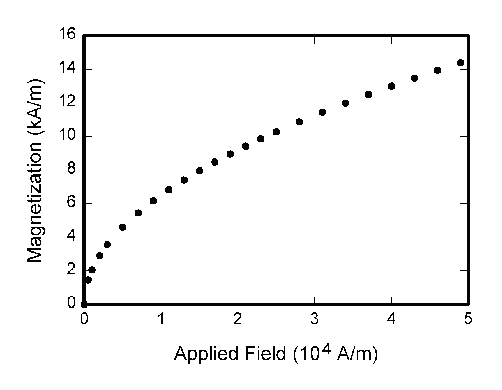
\includegraphics[scale=1]{field1.eps}
        \caption{Podajte kratko razlago slike.} \label{slika}
    \end{center}
\end{figure}

\section{Oddaja prispevka}

Prispevek oddajte v elektronski obliki preko formularja na spletni strani \cite{ERK}. Sprejemamo prispevke v formatu pdf (brez nastavljenih zaščitnih gesel) ali Microsoft Word. Pred oddajo prispevka prosimo preverite dodatne informacije za avtorje, ki so na spletnih straneh. 

Formular za elektronsko oddajo prispevkov bo aktiviran v juniju, rok za oddajo je \textbf{13. julij 2014}. Avtorje bomo obvestili o izboru konec avgusta.

\small
\begin{thebibliography}{1}

\bibitem{ERK} ERK, http://www.ieee.si/erk/index.html 
\bibitem{Zbornik} B. Zajc, A. Trost: Zbornik triindvajsete mednarodne Elektrotehniške in računalniške konference ERK 2014, 22. - 24. September 2014, Portorož, Slovenija

\end{thebibliography}

\end{document}
